\documentclass[12pt, twoside]{report}

\usepackage[utf8]{inputenc}
\def\magyarOptions{defaults=hu-min}
\usepackage[magyar]{babel}

\include{preamble}


\title{Bus4U - Szerver oldal}
\author{Zsigmond Attila}
\date{}

\begin{document}

\raggedbottom

\begin{titlepage}
  \centering
  \Large
  Sapientia Erdélyi Magyar Tudományegyetem \\
  Marosvásárhelyi Kar \\
  Számítástechnika szak \\
  \vspace{1.5in}
  \HUGE
  \textbf{Bus4U - Szerver oldal} \\
  \vspace{0.5in}
  \Huge
  \textbf{DIPLOMADOLGOZAT} \\
  \vspace{1.5in}
  \Large
  \begin{multicols}{2}
    \begin{flushleft}
      \textbf{Témavezető:} \\
      Ș.l.dr.ing. Szántó Zoltán
    \end{flushleft}
    \columnbreak
    \begin{flushright}
      \textbf{Hallgató:} \\
      Zsigmond Attila
    \end{flushright}
  \end{multicols}
  \vspace{0.5in}
  \LARGE
  2025
\end{titlepage}

\begin{titlepage}
  \centering
  \Large
  Universitatea „Sapientia” din Cluj-Napoca \\
  Facultatea de Științe Tehnice și Umaniste din Târgu-Mureș \\
  Specializarea Calculatoare \\
  \vspace{1.5in}
  \HUGE
  \textbf{Bus4U - Partea de Server} \\
  \vspace{0.5in}
  \Huge
  \textbf{PROIECT DE DIPLOMĂ} \\
  \vspace{1.5in}
  \Large
  \begin{multicols}{2}
    \begin{flushleft}
      \textbf{Coordonator științific:} \\
      Ș.l.dr.ing. Szántó Zoltán
    \end{flushleft}
    \columnbreak
    \begin{flushright}
      \textbf{Student:} \\
      Zsigmond Attila
    \end{flushright}
  \end{multicols}
  \vspace{0.5in}
  \LARGE
  2025
\end{titlepage}


\renewcommand{\abstractname}{Extras}
\begin{abstract}
  
Scopul aplicației web este de a face sistemele moderne de transport public mai prietenoase cu utilizatorul și mai eficiente, cu un accent deosebit pe planificarea călătoriilor, achiziționarea de bilete și urmărirea autobuzelor. Aplicația permite utilizatorilor să își planifice călătoriile în avans în cadrul rețelei de transport public dintr-un oraș sau o regiune specifică. Utilizatorii își pot achiziționa biletele pentru o rută selectată și pot vizualiza orele de plecare și sosire ale curselor, defalcat pe orașe și stații, asigurând astfel flexibilitate și informații de călătorie precise.

Aplicația oferă, de asemenea, o hartă interactivă care permite urmărirea în timp real a pozițiilor curente ale autobuzelor. Această funcție este deosebit de utilă atunci când apar schimbări neprevăzute în program, deoarece utilizatorii pot fi informați la timp despre întârzieri sau modificări ale traseelor. Pe lângă urmărirea în timp real, sistemul oferă locațiile geografice precise ale stațiilor de autobuz individuale, pe care utilizatorii le pot filtra în funcție de orașe sau rute, facilitând astfel planificarea la care stație să ajungă.

O aplicație separată care rulează pe terminalele POS aflate pe autobuze se ocupă de validarea biletelor și de partajarea continuă a pozițiilor autobuzelor cu serverul central, permițând utilizatorilor să rămână informați despre locațiile în timp real ale autobuzelor.

O altă componentă importantă a aplicației este interfața de administrare utilizată de companiile de autobuze. Această interfață permite gestionarea programelor, adăugarea de noi rute și stații și actualizarea datelor existente. În plus, informațiile despre angajați, inclusiv detaliile șoferilor și ale altui personal, precum și datele tehnice și de operare ale autobuzelor, pot fi gestionate aici. Acest sistem de administrare asigură funcționarea eficientă și întreținerea programelor, permițând companiilor de autobuze să își actualizeze cu ușurință serviciile și să asigure acuratețea.

Tema centrală a lucrării de diplomă este descrierea detaliată a componentelor serverului aplicației web, care asigură gestionarea fluidă a datelor utilizatorilor, a tranzacțiilor de achiziție a biletelor, a informațiilor de program și a urmării autobuzelor în timp real.

\vspace{1em}
\textbf{Cuvinte cheie:} transport public, urmărire în timp real, aplicație web, Rails API

\end{abstract}

\renewcommand{\abstractname}{Abstract}
\begin{abstract}
  
The purpose of the web application is to make modern public transportation systems more user-friendly and efficient, with a particular focus on trip planning, ticket purchasing, and bus tracking. The application allows users to plan their trips in advance within a specific city or region's public transportation network. Users can purchase tickets for a selected route and view the departure and arrival times of the services, broken down by cities and stops, thus ensuring flexibility and accurate travel information.

The application also offers an interactive map that allows real-time tracking of the current positions of buses. This feature is especially useful when unexpected changes occur in the schedule, as users can be timely informed about delays or route changes. In addition to real-time tracking, the system provides the precise geographical locations of individual bus stops, which users can filter based on cities or routes, making it easier to plan which stop to arrive at.

A separate application running on the POS terminals located on the buses ensures ticket validation and the continuous sharing of the buses' positions with the central server. This feature ensures that all participants in the system have up-to-date information, allowing users to stay informed about the real-time locations of the buses.

Another important component of the application is the administration interface used by the bus companies. This interface allows for the management of schedules, the addition of new routes and stops, and the updating of existing data. Additionally, employee information, including details of drivers and other staff, as well as technical and operational data of the buses, can be managed here. This administration system ensures efficient operations and schedule maintenance, enabling bus companies to easily update their services and ensure accuracy.

The central theme of the thesis is the detailed description of the server-side components of the web application, which ensure the seamless management of user data, ticket purchase transactions, schedule information, and real-time bus tracking.

\vspace{1em}
\textbf{Keywords:} public transportation, real-time tracking, web application, Rails API

\end{abstract}

\renewcommand{\abstractname}{Kivonat}
\begin{abstract}
  
A webalkalmazás célja a modern tömegközlekedési rendszerek felhasználóbaráttá és hatékonyabbá tétele, különös tekintettel az utazás megtervezésére, jegyvásárlásra, valamint az autóbuszok követésére. Az alkalmazás lehetővé teszi a felhasználók számára, hogy előre megtervezhessék utazásaikat egy adott város vagy régió tömegközlekedési hálózatán belül. A felhasználók megvásárolhatják jegyeiket egy kiválasztott járatra, valamint megtekinthetik a járatok indulási és érkezési időpontjait, városokra és megállókra bontva, biztosítva ezzel a rugalmasságot és a pontos utazási információkat.

Az alkalmazás egy interaktív térképet is kínál, amelyen valós időben nyomon követhetők az autóbuszok jelenlegi pozíciói. Ez a funkció különösen hasznos, amikor a menetrendben váratlan változások történnek, mivel a felhasználók időben értesülhetnek a késésekről vagy útvonal-módosításokról. A valós idejű követés mellett a rendszer biztosítja az egyes buszmegállók pontos földrajzi helyzetét, amelyeket a felhasználók városok vagy útvonalak alapján szűrhetnek, így könnyebben tervezhetik meg, melyik megállóhoz érkezzenek.

A buszokon található POS terminálokon futó különálló alkalmazás gondoskodik a jegyérvényesítésről és az autóbuszok pozíciójának folyamatos megosztásáról a központi szerverrel, így a felhasználók folyamatosan tájékozódhatnak az autóbuszok valós helyzetéről.

Az alkalmazás másik fontos része az adminisztrációs felület, amelyet a busztársaságok használhatnak. Ezen a felületen lehetőség van a menetrendek kezelésére, új útvonalak és megállók felvitelére, valamint a meglévő adatok frissítésére. Továbbá itt kezelhetők az alkalmazottak információi, beleértve a sofőrök és egyéb személyzet adatait, valamint az autóbuszok műszaki és üzemeltetési adatai. Ez az adminisztrációs rendszer biztosítja a hatékony működést és a menetrendek karbantartását, így a busztársaságok könnyedén frissíthetik szolgáltatásaikat és biztosíthatják a pontosságot.

A dolgozat központi témája a webalkalmazás szerver oldali komponenseinek részletes ismertetése, amelyek biztosítják a felhasználói adatok, a jegyvásárlási tranzakciók, a menetrendi információk, valamint a valós idejű autóbusz-követés zökkenőmentes kezelését.

\vspace{1em}
\textbf{Kulcsszavak:} tömegközlekedés, valós idejű követés, webalkalmazás, Rails API
\end{abstract}


\tableofcontents
\listoffigures

\chapter{Bevezető}

A modern világban a digitalizáció egyre inkább áthatja mindennapjainkat, a közlekedéstől kezdve a pénzügyi tranzakciókon át egészen az ügyintézésig. Az új technológiák bevezetése nem csupán kényelmesebbé, hanem hatékonyabbá és átláthatóbbá is teheti a különböző szolgáltatásokat. A tömegközlekedés területén azonban még mindig számos kihívással kell szembenéznünk, különösen a kisebb városokban és a regionális utazások során. Bár a nagyvárosokban egyre több helyen elérhető az elektronikus jegyrendszer és a valós idejű járatinformáció, sok vidéki térségben és távolsági közlekedési vonalon ezek a lehetőségek még mindig hiányoznak.

Az autóbuszok használata a közlekedés egyik leginkább környezetbarát formája, hiszen csökkenti a városi forgalmat és a szén-dioxid-kibocsátást. Ennek ellenére a buszközlekedés sokszor nem versenyképes alternatíva a magánautózással szemben, mivel a szolgáltatás minősége és elérhetősége gyakran nem felel meg a modern elvárásoknak. A jelenlegi rendszerek egyik legfőbb problémája a jegyvásárlási lehetőségek korlátozottsága: míg a városi közlekedésben már egyre inkább elérhető a bankkártyás és mobiltelefonos fizetés, a távolsági és regionális buszjáratok esetében sokszor még mindig csak készpénzzel lehet jegyet vásárolni a sofőrnél.

Egy másik fontos hiányosság, hogy sok esetben nem érhető el egy központi, megbízható információforrás a buszok menetrendjéről és aktuális helyzetéről. A buszmegállókban kifüggesztett menetrendek nem mindig naprakészek, és ha egy járat késik vagy kimarad, az utasoknak nincs lehetőségük arra, hogy erről időben értesüljenek. Egy digitális platform lehetőséget biztosíthatna a menetrendek valós idejű frissítésére, a buszok helyzetének követésére, valamint az utasok tájékoztatására késések esetén. Emellett sok felhasználó számára fontos lenne egy olyan alkalmazás, amely képes előre tervezni az utazásokat, például jegyfoglalási lehetőséggel vagy a járatok közötti átszállási lehetőségek figyelembevételével.

A jegyvásárlás és az utastájékoztatás digitalizálása nemcsak az utazók, hanem a busztársaságok számára is számos előnyt jelenthet. Az online jegyeladási rendszer segítségével pontosabb előrejelzések készíthetők az utasforgalomról, ami lehetővé teszi a járatok hatékonyabb üzemeltetését. Emellett a flottakezelési és adminisztrációs folyamatok is jelentősen egyszerűsíthetők egy digitális rendszer bevezetésével. Az autóbuszok műszaki állapotának és hivatalos dokumentumainak nyilvántartása papíralapon időigényes és kevésbé hatékony, míg egy online rendszer automatizált értesítésekkel segítheti a karbantartási és engedélyezési folyamatokat.

Fontos figyelembe venni azt is, hogy az utasok egyre nagyobb mértékben elvárják a digitális szolgáltatásokat, hiszen az okostelefonok és az internet folyamatos elérhetősége alapvetővé vált a mindennapi életben. Egy felhasználóbarát alkalmazás, amely egy helyen biztosítja az összes szükséges információt és lehetőséget a jegyvásárlásra, nemcsak kényelmesebbé teszi az utazást, hanem növeli is a tömegközlekedés iránti bizalmat. Az elmúlt években a digitális fizetési megoldások és az online utazástervezési eszközök iránti kereslet ugrásszerűen megnőtt, így a tömegközlekedési szolgáltatóknak is alkalmazkodniuk kell a változó utazási szokásokhoz.

A közlekedési rendszerek fejlesztése nem csupán technológiai kérdés, hanem társadalmi és környezetvédelmi szempontból is kiemelkedő jelentőséggel bír. A fenntartható közlekedési formák támogatása elengedhetetlen a nagyvárosi forgalmi dugók és a környezetszennyezés csökkentése érdekében. A buszközlekedés hatékonyabbá tétele és népszerűsítése hozzájárulhat a magánjármű-használat visszaszorításához, ezáltal mérsékelve a károsanyag-kibocsátást. Ha az emberek számára elérhetőbbé és megbízhatóbbá válik a tömegközlekedés, akkor nagyobb eséllyel választják azt a mindennapi utazásaik során, ami hosszú távon egy fenntarthatóbb városi mobilitást eredményezhet.

A rendszer két nagy részre osztható fel. Az egyik a frontend, amely a felhasználók számára látható felületeket, így a weboldalakat és a mobilalkalmazást tartalmazza, míg a másik rész a backend, amely az üzleti logikát, adatkezelést és API-végpontokat biztosítja. A backend részletes ismertetése az én dolgozatomban található meg, míg a frontend működését és implementációját külön dolgozat mutatja be \cite{bus4uui}.

Ebben a dolgozatban részletesen ismertetem a backend architektúrát, az API követelményeket, a technológiai választásokat, valamint az adatok tárolásának és kezelésének módját. Kitérünk a fejlesztés során alkalmazott tervezési döntésekre, a megvalósított funkciókra, továbbá a tesztelési módszerekre és a jövőbeni továbbfejlesztési lehetőségekre is. A dolgozat végén összegzem az eredményeket és levonom a projekt kapcsán szerzett tapasztalatokat.



\chapter{Célkitűzések}

A projekt célja, hogy egy modern, felhasználóbarát webalkalmazást fejlesszen ki a tömegközlekedés népszerűsítésére és a buszok használatának egyszerűsítésére. A következő konkrét célkitűzéseket határozzuk meg:

\begin{itemize}
    \item \textbf{Digitális Jegyvásárlás:} Olyan funkció kialakítása, amely lehetővé teszi a felhasználók számára, hogy előre jegyet vásároljanak a kívánt járatra, így csökkentve a készpénzes tranzakciók számát.
    
    \item \textbf{Valós Idejű Buszkövetés:} Integrálni egy valós idejű buszkövető rendszert, amely lehetővé teszi a felhasználók számára, hogy nyomon követhessék a buszok aktuális helyzetét és várható érkezési idejét.
    
    \item \textbf{Menetrendek Elérhetősége:} Biztosítani, hogy a buszmenetrendek minden megállóban könnyen elérhetők legyenek, valamint online platformon is megtekinthetők legyenek.
    
    \item \textbf{Interaktív Térkép:} Fejleszteni egy interaktív térképet, amely lehetővé teszi a felhasználók számára, hogy könnyen navigáljanak a város tömegközlekedési hálózatán, és információkat kapjanak a megállókról és járatokról.
    
    \item \textbf{Adminisztrációs Felület:} Létrehozni egy adminisztrációs felületet, amelyet a busztársaságok használhatnak a menetrendek, útvonalak és alkalmazottak információinak kezelésére, ezzel növelve a működés hatékonyságát.
    
    \item \textbf{Felhasználói Élmény Javítása:} A webalkalmazás tervezése során a felhasználói élmény maximalizálása, beleértve a könnyű navigációt és az intuitív felület kialakítását.
\end{itemize}

Ezek a célkitűzések a webalkalmazás fejlesztésének alapját képezik, és hozzájárulnak a modern tömegközlekedési rendszerek hatékonyabbá tételéhez, valamint a felhasználók utazási élményének javításához.


\chapter{Elméleti megalapozás és bibliográfiai tanulmány}
\section{Technológiai háttér}
A Bus4U alkalmazás digitális megoldásai mögött modern webtechnológiák állnak, amelyek lehetővé teszik a felhasználói élmény folyamatos fejlesztését és a szolgáltatások hatékony működését. Az alkalmazás backendje Ruby on Rails keretrendszert használ, amely az egyik legnépszerűbb választás webes alkalmazások fejlesztésére.

\subsection{Ruby on Rails}
A \textit{Ruby on Rails} egy népszerű és széles körben használt webes keretrendszer, amely a Ruby programozási nyelvre épül. A Rails két alapvető elv alapján működik: a „\textit{Convention over Configuration}” és a „\textit{Don’t Repeat Yourself}”. Ezek az elvek azt eredményezik, hogy a fejlesztőknek kevesebb kóddal kell dolgozniuk, mivel a Rails konvenciói automatikusan meghatározzák a konfigurációkat, így csökkentve a redundáns kódot és növelve a fejlesztési folyamat hatékonyságát \cite{hartl_rails, fernandez_rails}. Ez különösen hasznos nagyobb projektek esetén, mivel elősegíti a gyorsabb fejlesztést és az egyszerűbb karbantartást, amely a gyorsan változó üzleti igények mellett nélkülözhetetlen.

A Rails \textit{MVC (Model-View-Controller)} architektúrára épül, amely logikailag elkülöníti az alkalmazás különböző részeit: az adatkezelést (Model), a felhasználói felületet (View), és az üzleti logikát (Controller). Ez a struktúra átláthatóbbá teszi a kódot, mivel a különböző funkciók külön-külön karbantarthatók, anélkül hogy zavarnák egymást, valamint megkönnyíti az új funkciók hozzáadását is. A Rails alkalmazásokhoz számos „\textit{gem}”, vagyis könyvtár érhető el, amelyek előre elkészített megoldásokat kínálnak, így még a komplexebb funkciók integrálása is könnyebb és biztonságosabb lehet \cite{hartl_rails}.

A Rails további előnye, hogy natív módon támogatja \textit{RESTful API}-k létrehozását. A RESTful megközelítés egyértelmű, szabványosított formát biztosít az API-k számára, amely megkönnyíti az alkalmazások közötti integrációt, például egy mobilalkalmazás és a backend közötti kommunikáció során. Ennek a felépítésnek köszönhetően a Rails alkalmazások egyszerűen összekapcsolhatók más rendszerekkel és frontend megoldásokkal \cite{fernandez_rails}.

Végül, a Rails beépített tesztelési eszközei lehetőséget adnak az automatizált tesztelésre, amely hozzájárul a szoftverek magasabb megbízhatóságához és a hibamentes működés biztosításához a fejlesztés minden szakaszában. Az ilyen automatizált tesztelési funkciók szintén csökkentik a karbantartási költségeket, hiszen a kódminőség magasabb szinten tartható, és gyorsan azonosíthatók a hibák \cite{hartl_rails, fernandez_rails}.

\subsection{PostgreSQL}
A \textit{PostgreSQL} egy \textit{nyílt forráskódú, objektum-relációs adatbázis-kezelő rendszer}, amely széles körben ismert teljesítményéről, rugalmasságáról, és különösen alkalmas komplex adatszerkezetek és nagy adattömegek kezelésére. Támogatja a fejlett adattípusokat, bonyolult lekérdezéseket, és párhuzamos műveleteket, amelyek különösen hasznosak a Bus4U-hoz hasonló, valós idejű adatokat feldolgozó rendszerekben \cite{douglas_postgresql, murrell_postgresql}.

A PostgreSQL előnyei a Bus4U számára: \begin{itemize} \item \textbf{Teljesítmény optimalizálása és bonyolult lekérdezések kezelése}: A PostgreSQL kiválóan kezeli a párhuzamos lekérdezéseket és optimalizált módon képes kezelni nagy mennyiségű adatot és komplex lekérdezési struktúrákat. Ez biztosítja az alkalmazás gyors, megbízható működését, és lehetőséget nyújt az adatbázis hatékony méretezésére és finomhangolására az adatmennyiség növekedésével \cite{murrell_postgresql}. \item \textbf{Skálázhatóság}: Nagyobb adatmennyiség vagy felhasználói terhelés esetén a PostgreSQL támogatja a függőleges és vízszintes skálázást. Ezen túlmenően replikációval biztosítható a magas rendelkezésre állás, amely kritikus szempont a nagy terhelés alatt működő rendszerekben. Így a PostgreSQL hosszú távú, fenntartható teljesítményt és magas rendelkezésre állást biztosít, amely elengedhetetlen a Bus4U megbízható működéséhez \cite{douglas_postgresql}. \end{itemize}

\subsection{Azure}
Az \textit{Azure} egy olyan nagyvállalati szintű, biztonságos és skálázható felhőplatform, amely számos lehetőséget kínál modern alkalmazások fejlesztéséhez és működtetéséhez. Az Azure infrastruktúrája révén biztosítható a folyamatos és megbízható működés, míg a platform rugalmassága lehetővé teszi az erőforrások hatékony kezelését és a skálázhatóságot \cite{wilder_azure, collier_azure}. Az Azure használatával elkerülhetőek a hagyományos szerver infrastruktúrák fizikai korlátai, és olyan erőforrások válnak elérhetővé, amelyek az alkalmazás igényei szerint rugalmasan méretezhetők.

Az Azure előnyei a Bus4U számára:

\begin{itemize} 
    \item \textbf{Skálázhatóság és rugalmasság}: Az Azure automatikusan alkalmazkodik a változó terheléshez, amely lehetővé teszi, hogy a rendszer gördülékenyen kezelje a megnövekedett felhasználói forgalmat. Ez az adaptív megközelítés egy modern, folyamatosan növekedő alkalmazás számára elengedhetetlen, különösen tömegközlekedési rendszerek esetében, ahol a felhasználói igények időben változhatnak \cite{wilder_azure}.
    \item \textbf{Biztonság és adatvédelem}: Az Azure erőteljes adatvédelmi szabályokat és fejlett biztonsági protokollokat alkalmaz. Ezek közé tartozik a többfaktoros hitelesítés, a hálózati tűzfalak, valamint az adattitkosítás, amelyek biztosítják, hogy a Bus4U felhasználóinak adatai biztonságban legyenek. A platform megfelel a szigorú adatvédelmi szabványoknak, ami kulcsfontosságú egy olyan alkalmazás számára, amely szenzitív felhasználói adatokat kezel \cite{collier_azure}.
\end{itemize}

\section{A közlekedési rendszerek és a jövőbeli trendek}

A közlekedési rendszerek jövőbeli fejlődése alapvetően meghatározza az olyan alkalmazások, mint a Bus4U sikerét. Levinson és Krizek \cite{levinson_transport} szerint a közlekedés jövője radikális változások elé néz, amelyek magukban foglalják a forgalom csökkenését és az új mobilitási megoldások elterjedését. A közlekedés jövőjére vonatkozó előrejelzések hangsúlyozzák az automatizálás, a megosztott közlekedési módok és az okos városok integrálását, amelyek mind hozzájárulnak a fenntarthatóbb és hatékonyabb közlekedési hálózatok kialakításához. A Bus4U alkalmazás azzal, hogy valós idejű információkat biztosít a közlekedési rendszerről, közvetlenül hozzájárulhat ezen trendek előmozdításához.

Ceder \cite{ceder_transit} a közlekedési rendszerek tervezésében és üzemeltetésében alkalmazott eljárásokat és módszereket vizsgálja, különös figyelmet fordítva a tömegközlekedési rendszerek hatékonyságának és minőségének javítására. Az alkalmazás szempontjából kulcsfontosságú lehet, hogy a különböző típusú közlekedési eszközök integrálása és azok közötti interakciók optimalizálása révén a rendszer a lehető legjobb utazási élményt biztosítsa. Az automatizált jegyvásárlás és az utazási időszámítás optimalizálása mind hozzájárulhat a felhasználók elégedettségéhez.

\section{Hasonló alkalmazások}

A közlekedési alkalmazások, mint például a Budapest Go, jelentős hatással vannak a modern városi közlekedésre. A Budapest Go a magyarországi főváros tömegközlekedési rendszerének digitális megoldása, amely lehetővé teszi a felhasználók számára, hogy egyszerűen és gyorsan intézzék utazásaik szervezését. Az alkalmazás számos funkcióval rendelkezik, amelyek javítják a felhasználói élményt.

A Budapest Go célja, hogy a város tömegközlekedését még hozzáférhetőbbé és felhasználóbarátabbá tegye. Az alkalmazás főbb jellemzői közé tartozik:

\begin{itemize} \item Valós idejű menetrendek: Az alkalmazás folyamatosan frissíti a buszok, villamosok és metrók érkezési idejét, lehetővé téve a felhasználók számára, hogy pontosan tudják, mikor indul a következő járat. \item Online jegyvásárlás: A felhasználók az alkalmazáson belül jegyeket vásárolhatnak, ami gyorsítja a folyamatot és csökkenti a sorban állás szükségességét. \item Útvonaltervezés: Az alkalmazás lehetővé teszi a felhasználók számára, hogy megtervezzék utazásaikat, figyelembe véve a különböző közlekedési eszközöket és a lehető leghatékonyabb útvonalakat. \item Használati statisztikák: A Budapest Go elemzi a felhasználók utazási szokásait, lehetővé téve a szolgáltatók számára, hogy jobban megértsék a közlekedési igényeket és fejleszthessék szolgáltatásaikat. \end{itemize}

\subsection{Felhasználói élmény és innovációk}

A Budapest Go nemcsak a közlekedési információk egyszerűsítésére szolgál, hanem innovatív megoldásokat is kínál a felhasználók számára. Az alkalmazás intuitív felhasználói felülete lehetővé teszi a könnyű navigációt, így még a technológiához kevésbé értő felhasználók is könnyen el tudnak igazodni.

\subsection{Hatások a közlekedési rendszerre}

A Budapest Go alkalmazás bevezetése jelentős hatással volt a főváros közlekedési rendszerére. A digitális jegyvásárlás elterjedése csökkentette a készpénzes tranzakciók számát, így gyorsabbá téve a közlekedési folyamatokat. Ezenkívül a valós idejű információk elérhetősége segít a felhasználóknak a jobb döntéshozatalban, ami hozzájárul a város közlekedési hatékonyságának növeléséhez.

A Budapest Go egy példa arra, hogyan lehet a digitális technológiát alkalmazni a városi közlekedés fejlesztésére. Az alkalmazás által kínált funkciók és a felhasználói élmény folyamatos javítása hozzájárul a közlekedési rendszerek modernizálásához és a fenntartható közlekedés népszerűsítéséhez.

\chapter{Rendszer specifikációi}

\section{Felhasználói követelmények}
A felhasználói weboldal bejelentkezés nélkül használható. A főoldalon lehetőség nyílik rákeresni járatokra dátum, idő és cél alapján, a menetrendeknél megtekinthetőek a buszok és a megállók órarendjei. A megállók oldalon megjelenik az összes megálló a térképen, amelyek között szűrést is lehet alkalmazni. Az élőben frissülő térkép lapon követni lehet a buszok pozícióját percről percre. A jegyek oldalon vannak listázva az eddig megvásárolt jegyek QR-kódjai, a rólunk szóló oldalon pedig egy rövid leírás található a projektről. Fiókot létrehozni kizárólag a jegyvásárláshoz szükséges, ami a főoldalon lehetséges amennyiben a felhasználó megtalálta a neki megfelelő járatot és rálépett a vásárlás gombra. Fiók regisztrációjához meg kell adni a teljes nevet, egy meglévő email címet, egy új jelszót, majd egy ellenőrző kódot, amit a rendszer elküld a megadott email címre.

Az admin felület kizárólag bejelentkezéssel elérhető, új fiókokat pedig csak az adott cég főnöke tud létrehozni a saját busztársaságához, erre az alkalmazottak című lapon van lehetőség. Emellett az adminoknak lehetőségük van szerkeszteni a megállók listáját, valamint az útvonalak összes tulajdonságát is (meglátogatott megállók, indulási időpontok és jegyárak), ezeket a megállóknak és a járatoknak szóló oldalakon. A főoldalon egy statisztikát is láthatnak az eladott jegyek számáról, a megtett kilométerről és a bevételről, mindezt hónapos, éves és mindenkori bontásokban. Van még egy lap a buszok adatainak kezelésére is, ahol lehet konfigurálni az útadót, a biztosítást és a műszaki vizsgát is, valamit itt lehet buszokat kivonni forgalomból és hozzáadni újakat is.

A Flutter alapú mobil applikáció ugyanúgy működik, mint a felhasználóknak szánt weboldal, így ugyanazok a követelmények vonatkoznak erre is.

A POS terminál alkalmazás használatához szükség van egy sofőr szerepkörű admin fiókra. Bejelentkezés után lehetőség van egy adott busz követését, illetve a jegyszkennelő programot elindítani.

\section{Rendszerkövetelmények}

\subsection{Funkcionális követelmények}
A felhasználói felület minden oldalán van egy kis form, amelyet kitöltve le lehet kérni az adatbázisból az adott oldalon megjelenítendő adatokat. Ilyenre példa van a főoldalon is, ahol meg kell adni az indulás helyét, a cél helyét (települést) és opcionálisan az ezekhez tartozó megállót, egy-egy lenyíló listából kiválasztva az adatokat. A települések betöltődnek az oldallal együtt, a megállók listája viszont csak a város kiválasztása után, mindig csak az adott településen találhatóak jelennek meg. Ezen kívül a főoldalon van egy dátumválasztó és egy időválasztó is, ezek alapértelmezetten az aktuális dátummal és idővel vannak kitöltve. Ha a form ki van töltve, a keresés gomb lenyomására az oldal elküldi a bevitt adatokat a backend szerverre, amely válaszként elküld egy listát a megfelelő utazási lehetőségekkel. Ezek az adatok JSON formátumban, HTTP protokollon keresztül közlekednek a frontend és backend között. A többi oldal is hasonlóan működik, először az adatokat kell megadni, aztán a gomb lenyomására pillanatok alatt megjelenik a képernyőn a szerver válasza a bevitt adatokra.

A különböző formokon kívül, a weboldalon található térképek is API hívásokkal működnek. A rendszer először betölti az alap térképet a MapBox API segítségével, aztán amint a felhasználó kiválasztotta a megtekinteni kívánt útvonalat a Menetrend vagy az Élő térkép lapon, a weboldal a saját adatbázisunkból kéri le a hozzá tartozó megállók koordinátáit, ezeket megjeleníti a térképen, végül ismét a MapBox API-t használva útvonal-tervet generáltat. Ez úgy működik, hogy a rendszer elküldi a megállók listáját és visszakap egy sok pontból álló új listát a MapBox-tól, ezeket összekötve sok kis vonallal, kirajzolódik a részletes útvonal a térképen.

\subsection{Nem-funkcionális követelmények}

\paragraph{Szervezéssel kapcsolatos követelmények}
\begin{itemize}
    \item Programozási nyelvek: Ruby, Dart, HTML, CSS, JavaScript
    \item Keretrendszerek: Ruby on Rails, Flutter, Vue.js
    \item IDE: Visual Studio Code
    \item Verziókövetés: Git és GitHub
    \item Adatbázis: Postgres
    \item Cloud Service: Azure
    \item Webhost: Netlify
    \item Csoportos kommunikáció: Slack
\end{itemize}

\paragraph{Termékkel kapcsolatos követelmények}
A felhasználói weboldal és az admin felület használatához egy modern, internetezésre alkalmas eszközre van szükség. Ajánlott a 2018 után kiadott böngészők használata:
\begin{itemize}
    \item Chrome >= 87
    \item Firefox >= 78
    \item Safari >= 14
    \item Edge >= 88
\end{itemize}

Az applikáció használatához szükség van egy okostelefonra, vagy tabletre, amelyen minimum Android 5 vagy iOS 8-as verzió van telepítve. Fontos, hogy legyen rajta helymeghatározás, internet elérés (3G, 4G, 5G) és legyen rajta minimum 120MB szabad tárhely és 516-1024 MB szabad memória.

A POS terminál alkalmazásához ideális esetben egy Sunmi V2 PRO típusú POS terminálra van szükség, de ha ez valamilyen oknál fogva nem áll rendelkezésre, akkor bármilyen, legalább Android 5.0-át, vagy iOS 8-at futtató, kamerával és GPS antennával rendelkező eszköz megteszi, illetve szükség van 100MB szabad tárhelyre és 510MB szabad memóriára.



\chapter{A rendszer részletes leírása}
Rendszerünk öt fő komponensből áll, amelyeket a komponens diagramon is láthatunk: egy Ruby on Rails keretrendszerben írt API-ból, egy Vue.js alapú webes felhasználói- és admin felületből, egy Flutter alkalmazásból a felhasználók számára, valamint egy Flutter keretrendszerben készült POS terminál alkalmazásból. Az API a REST architektúrát követi, lehetővé téve a különböző erőforrások, például buszok, járatok és jegyek kezelését. A felhasználói és admin weboldal Vue-ban készült, a Vuetify elemek felhasználásával, ami lehetővé tette az egyszerű és hatékony felhasználói felületek gyors fejlesztését. A Vue.js keretrendszer előnye, hogy komponensekből áll, így átlátható és jól rendszerezett webalkalmazás felépítést tesz lehetővé. Ezen kívül a Vuetify komponens-készlete megkönnyítette az UI elemek létrehozását, gyorsítva ezzel a fejlesztési folyamatot. Az alkalmazás Flutterben készült, Dart programozási nyelvet használva, amely lehetővé teszi, hogy ugyanazt a kódbázist használjuk iOS és Android platformokra is, így jelentősen csökkentve a fejlesztési időt és költségeket. A POS terminál alkalmazása is Flutter keretrendszerben készült, biztosítva a hatékony és egységes megoldást a különböző platformok számára.
A Vue.js alapú weboldalakat, illetve a felhasználóknak szánt Flutter alkalmazást Portik Szabolcs kollegám mutatja be részletesebben egy másik dolgozat 
keretein belül.

\begin{figure}[H]
    \centering
    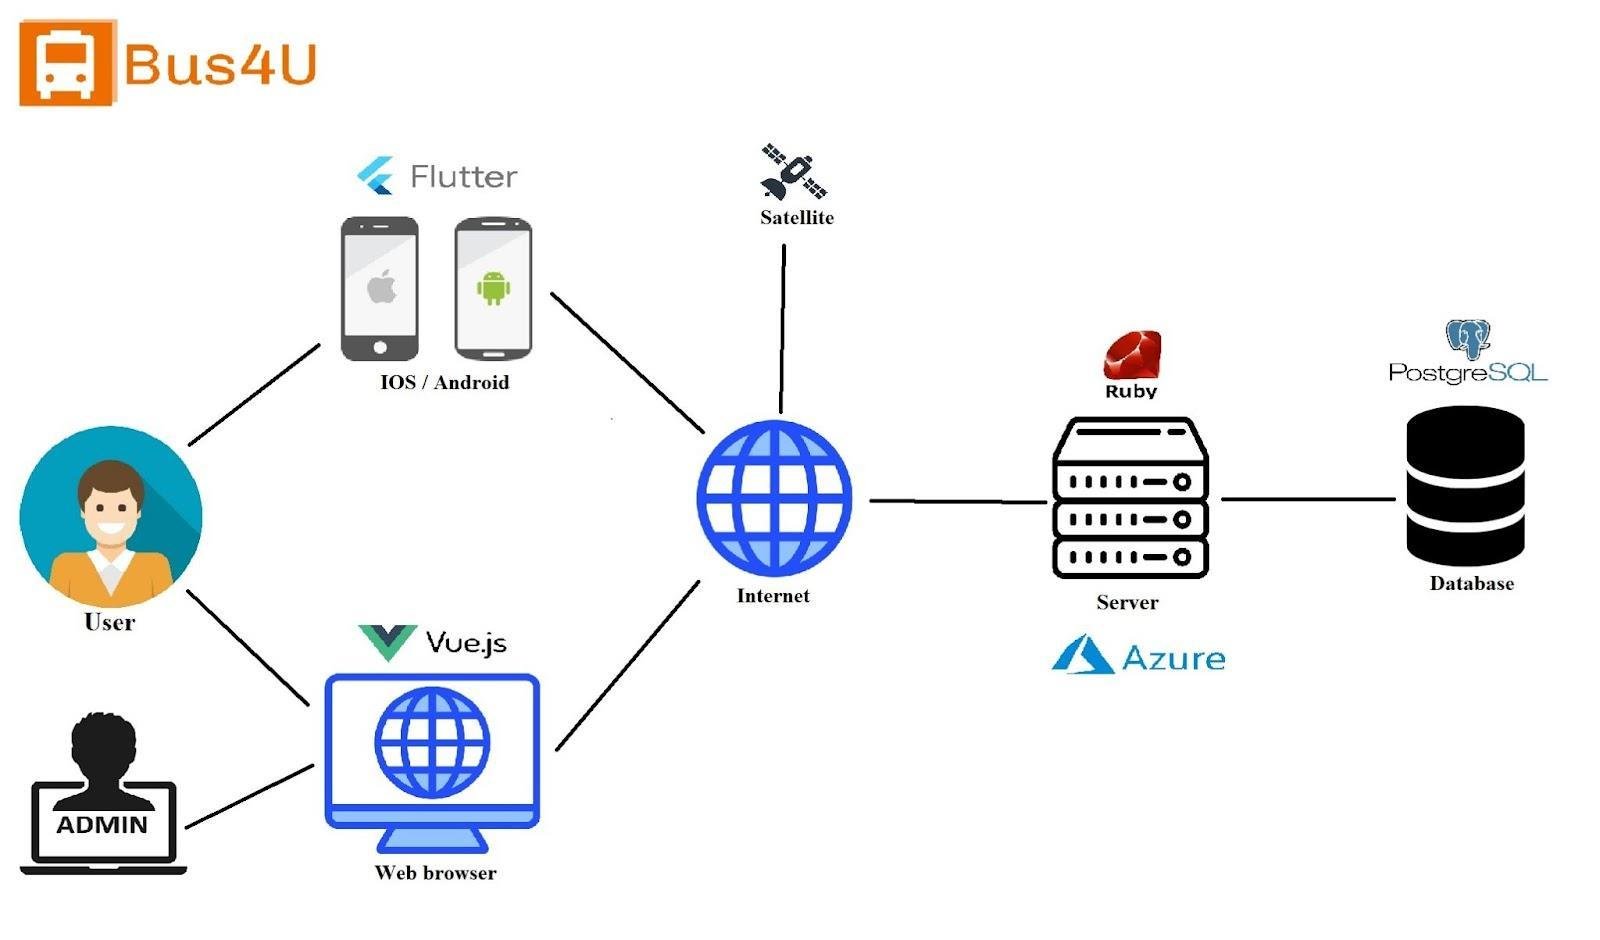
\includegraphics[width=\textwidth]{figures/component.jpg}
    \caption{A rendszer komponensdiagramja}
    \label{fig:component-diagram}
  \end{figure}


\section{Az API felépítése}
A Bus4U API a REST architektúrát követi, és számos végpontot biztosít a különböző erőforrások kezeléséhez, mint például:
\begin{itemize}
    \item \textbf{Buszok kezelése}: buszok létrehozása, frissítése, törlése.
    \item \textbf{Járatok menedzselése}: járatok lekérése és ütemezése.
    \item \textbf{Jegyek és bérletek}: jegyek és bérletek vásárlása és kezelése.
\end{itemize}

\section{Endpointok részletes leírása}

\subsection{GET /get\_stations\_by\_city}
Ez az endpoint lehetővé teszi a megállók listájának lekérését egy adott város alapján. A kérés a következő paramétert használja:
\begin{itemize}
    \item \textbf{city\_uid}: A város egyedi azonosítója.
\end{itemize}

\textbf{Példa kérés}:
\begin{verbatim}
GET https://api.bus4u.online/v1/get_stations_by_city?city_uid=CTY_N11XH
\end{verbatim}

\textbf{Válasz formátum}:
\begin{verbatim}
{
    "stations": [
        {
            "station_uid": "STT_EGAVX",
            "name": "Sapientia",
            "address": "Str. Calea Sighisoarei nr. 2",
            "longitude": "24.59883",
            "latitude": "46.52339"
        },
        {
            "station_uid": "STT_6CO3Q",
            "name": "Dedeman",
            "address": "Bul. 1 Decembrie nr. 189",
            "longitude": "24.59941",
            "latitude": "46.52678"
        }
    ]
}
\end{verbatim}

\section{Adatkezelés és adatbázis kapcsolat}
Az API végpontjai a \textbf{PostgreSQL} adatbázissal kommunikálnak. Az adatbázis tranzakciókat az \textbf{ActiveRecord} ORM segítségével kezeljük, amely lehetővé teszi az adatok egyszerű és hatékony lekérését, beszúrását és frissítését.

\subsection{Adatbázis táblák}
A PostgreSQL adatbázisunk a következő táblákból áll:
\begin{itemize}
    \item \textbf{Companies}: Azon cégek adatai, akikkel szerződést kötött a Bus4U.
    \item \textbf{Admins}: Különböző cégekhez tartozó adminisztrátorok adatai. Szerepük lehet “boss” vagy “driver”.
    \item \textbf{Buses}: A cégekhez tartozó autóbuszok adatai.
    \item \textbf{Routes}: A cégek saját útvonalai.
    \item \textbf{Stations}: A rendszerben található buszmegállók összessége.
    \item \textbf{Route\_stations}: Egy cég adott útvonalán keresztülhaladó megállók.
    \item \textbf{Timetables}: Egy útvonal megállójának indulási időpontjai és ára nap szerinti felosztásban.
    \item \textbf{Cities}: Az összes város, amelyen áthaladnak útvonalak.
    \item \textbf{Users}: A Bus4U felhasználói a fontosabb adataikkal.
    \item \textbf{Email\_verifications}: Az adott email címekhez tartozó regisztrációkor felhasználandó kódok.
    \item \textbf{Tickets}: A felhasználókhoz tartozó jegyek.
    \item \textbf{Payments}: Stripe fizetések eltárolása.
\end{itemize}

\begin{figure}[H]
    \centering
    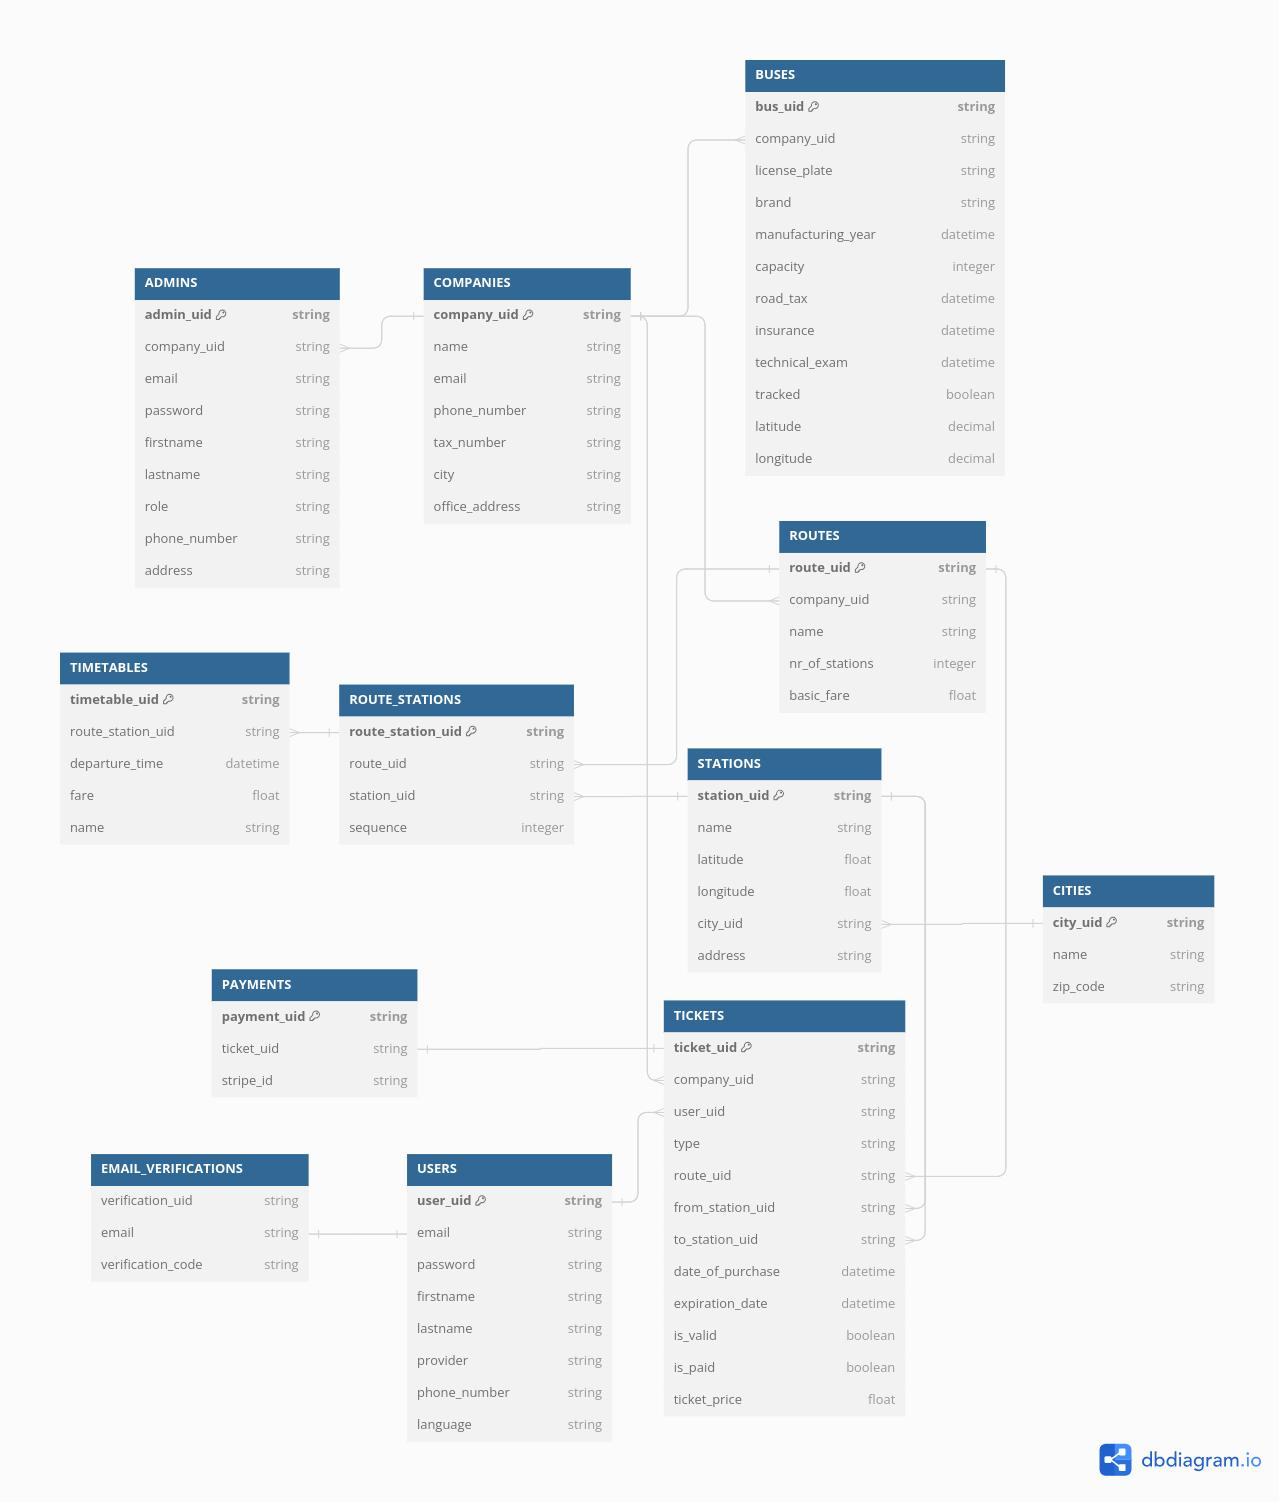
\includegraphics[width=\textwidth]{figures/database.jpg}
    \caption{Az rendszer adatbázisdiagramja}
    \label{fig:database-diagram}
  \end{figure}

  \section{Projektmenedzsment és verziókövetés}

  A projekt fejlesztése során több eszközt alkalmaztunk a feladatok nyomon követésére, a fejlesztési folyamat szervezésére és a forráskód verziókövetésére.
  
  \subsection{Jira}

  A projektmenedzsment során a \textbf{Jira} kanban boardját használtuk, amely az Atlassian által fejlesztett projekt-követő platform. A Jirát választottuk, mert egy olyan hatékony eszköz, amely egyszerre letisztult, ám funkciókban komplex, így könnyedén igazítható a projekt igényeihez. 
  
  A Kanban tábla három fő oszlopból állt:
  \begin{itemize}
      \item \textbf{To do}: Ide kerültek azok a feladatok, amelyeket még nem kezdtünk el.
      \item \textbf{In progress}: Ebben az oszlopban azok a feladatok szerepeltek, amelyek éppen folyamatban voltak.
      \item \textbf{Done}: Az elvégzett feladatok ebbe az oszlopba kerültek, jelezve azok befejezését.
  \end{itemize}
  
  Minden feladatot hozzárendeltünk egy konkrét tulajdonoshoz, valamint címkékkel láttunk el, amelyek megjelölték, hogy a munka épp a rendszer melyik komponensére vonatkozik: \textbf{API}, \textbf{felhasználói felület}, \textbf{admin felület}, vagy \textbf{mobil alkalmazás}. A feladatok ilyen címkézése segített abban, hogy pontosan tudjuk, ki mivel foglalkozik, illetve milyen állapotban van a fejlesztés különböző területein végzett munka.

  \begin{figure}[H]
    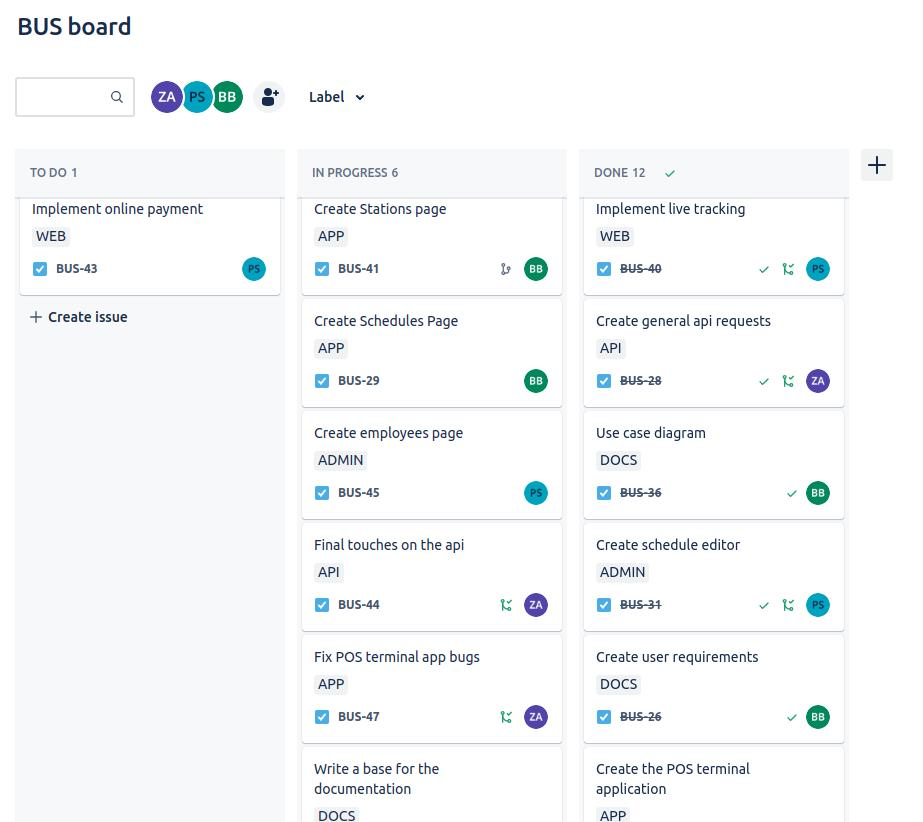
\includegraphics[width=\textwidth]{figures/jira.jpg}
    \caption{A Jira kanban board áttekintése}
    \label{fig:jira}
  \end{figure}
      
  \subsection{Git és GitHub}

  A projekt forráskódjának verziókezelését a \textbf{Git} verziókezelő rendszer segítségével oldottuk meg, míg a kód tárolására a \textbf{GitHub} platformot használtuk. A GitHub lehetőséget biztosított a pull request-ek hatékony kezelésére, amelyekkel minden változtatást egyszerűen tudtunk jóváhagyni. Ez a megközelítés a kód visszakövethetőségét és dokumentálását is jelentősen megkönnyítette, hozzájárulva a kód minőségének javításához és a fejlesztési folyamat átláthatóságához.
  
  A projekt struktúráját három fő \textbf{branch} köré szerveztük:
  \begin{itemize}
      \item \textbf{main branch}: Ebbe az ágba kizárólag a már teljesen tesztelt és stabil kódrészletek kerültek be, amelyeket időszakosan publikáltunk. Ez az ág szolgált a hivatalos, működőképes verzió tárolására.
      \item \textbf{develop branch}: A develop branch-et a fejlesztés és tesztelés helyszíneként használtuk. Az ide feltöltött kódok még tesztelés alatt álltak, de a fejlesztési idő alatt mindig a develop verzióját futtattuk az Azure környezetben, ezzel biztosítva, hogy az aktuális fejlesztések folyamatosan elérhetők és tesztelhetők legyenek.
      \item \textbf{feature branchek}: Az új funkciók fejlesztését különálló, ún. feature branchekben végeztük, amelyek a konkrét feladatokra vagy kódrészletekre koncentráltak. Például kisebb munkaigényű kódok, mint az általános API lekérések fejlesztése külön branchekben történt, míg az összetettebb funkciókat külön feature branch-ekben dolgoztuk ki.
  \end{itemize}
  
  A branch-ek ilyen felosztása lehetővé tette a párhuzamos fejlesztést, és biztosította, hogy a különböző fejlesztési szakaszok kódjai elkülönítve és rendezetten legyenek tárolva. A GitHub pull request funkciójának köszönhetően minden változtatást felül tudtunk vizsgálni, így minden módosítás előtt biztosak lehettünk annak minőségében és kompatibilitásában.

  \begin{figure}[H]
    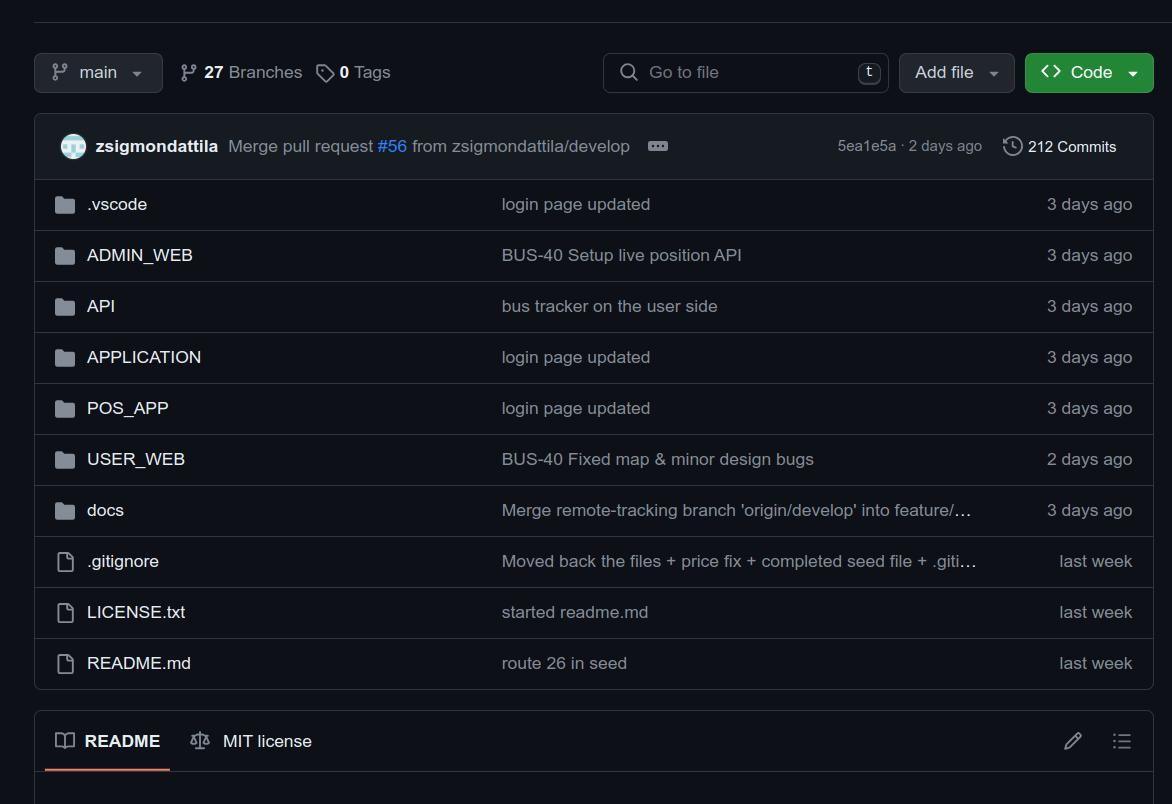
\includegraphics[width=\textwidth]{figures/github.jpg}
    \caption{A GitHub repository áttekintése}
    \label{fig:github}
  \end{figure}
  
  
  Ezek az eszközök hozzájárultak a projekt sikeres és hatékony fejlesztéséhez, elősegítve a feladatok egyértelműsítését, priorizálását és a csapat tagjai közötti együttműködést.
  


\chapter{Infrastruktúra}
\section{Azure infrastruktúra áttekintése}
A Bus4U rendszer a Microsoft Azure felhőalapú platformján került telepítésre. Az Azure szolgáltatások skálázhatóságot és megbízhatóságot biztosítanak a rendszer számára. A telepítéshez az alábbi főbb szolgáltatásokat használtam:
\begin{itemize}
    \item \textbf{Azure Virtual Machines (VM)}: A szerver hosztolása.
    \item \textbf{Azure Database for PostgreSQL}: Az adatbázis-szolgáltatás biztosítása.
\end{itemize}

\section{Domain konfiguráció}
A rendszer az \textbf{api.bus4u.online} domainen érhető el, amelyet a Cloudflare platformján konfiguráltam. A domain hozzárendelése során a virtuális gép (VM) IP címét használtam. A következő beállításokat végeztem el:
\begin{itemize}
    \item \textbf{DNS beállítások}: A Cloudflare-en elvégeztem a domain névhez tartozó A és CNAME rekordok konfigurálását.
    \item \textbf{SSL tanúsítványok}: A HTTPS alapú kapcsolat biztonságának érdekében a Cloudflare szolgáltatásait alkalmazzuk, amelyek védelmet nyújtanak a felhasználók számára.
\end{itemize}


\section{Adatbázis telepítése és konfigurációja}
A rendszer adatbázisa egy \textbf{Azure Database for PostgreSQL} szolgáltatáson keresztül került telepítésre, amely lehetővé teszi az adatbázis automatikus méretezését és a folyamatos biztonsági mentések készítését. A következő beállításokat alkalmaztuk:
\begin{itemize}
    \item \textbf{Titkosított kapcsolatok}: A PostgreSQL adatbázis SSL tanúsítványokat használ a biztonságos kommunikációhoz.
    \item \textbf{Backup és recovery}: Automatikus biztonsági mentések kerülnek tárolásra az adatvesztés elkerülése érdekében.
\end{itemize}

\section{Szerver telepítése}
A szerver az \textbf{Azure Virtual Machines} szolgáltatásban került telepítésre, ahol a Ruby on Rails alapú API-t futtatjuk. A telepítés során a következő lépéseket hajtottuk végre:
\begin{itemize}
    \item \textbf{Környezeti változók beállítása}: A szükséges konfigurációs változók (pl. adatbázis kapcsolatok) a Ruby on Rails beépített credentials funkciójában lettek biztonságosan tárolva és kezelve.
    \item \textbf{Verziókezelés}: Az \textbf{asdf} verziókezelő használatával a Ruby és egyéb nyelvek verzióit könnyen kezelhetjük, ami megkönnyíti a fejlesztési környezet fenntartását.
    \item \textbf{CI/CD pipeline}: Az alkalmazás automatikus telepítése és frissítése a GitHub Actions integrációjával valósult meg.
\end{itemize}

\begin{figure}[H]
    \centering
    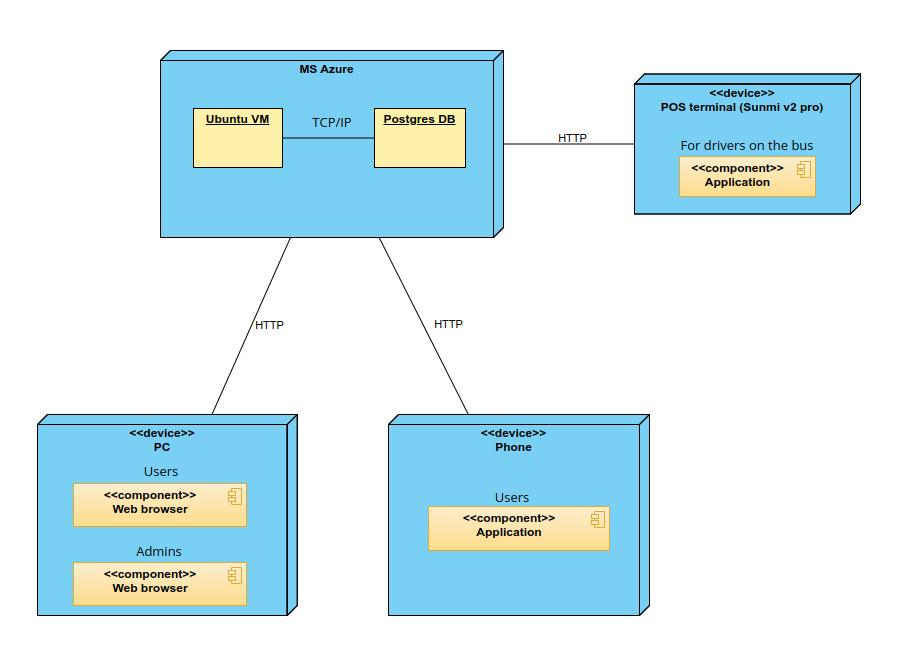
\includegraphics[width=\textwidth]{figures/deployment.jpg}
    \caption{Telepítési diagram}
    \label{fig:deployment-diagram}
  \end{figure}

\chapter{Az alkalmazás működése}
\section{Felhasználói felület}
\subsection{Főoldal}
A weboldalra rákeresve a felhasználót a kezdőoldal fogadja, ahol lehetőség van
egy utazás megtervezésére. Ki kell választani a kiindulási helyet és megállót, majd a
célt, az utazás dátumát és időpontját. Ekkor a rendszer lekéri a szerverről a megadott
megállók közötti, az adott napon, a megadott időpont után közlekedő járatokat és azok
jegyárát. Minden egyes járatnál van egy vásárlás gomb, amellyel a felhasználó
megszerezheti a jegyet vagy jegyeit az adott buszjáratra, amennyiben be van
jelentkezve, ellenkező esetben a rendszer átirányítja a bejelentkezéshez.

\begin{figure}[H]
    \centering
    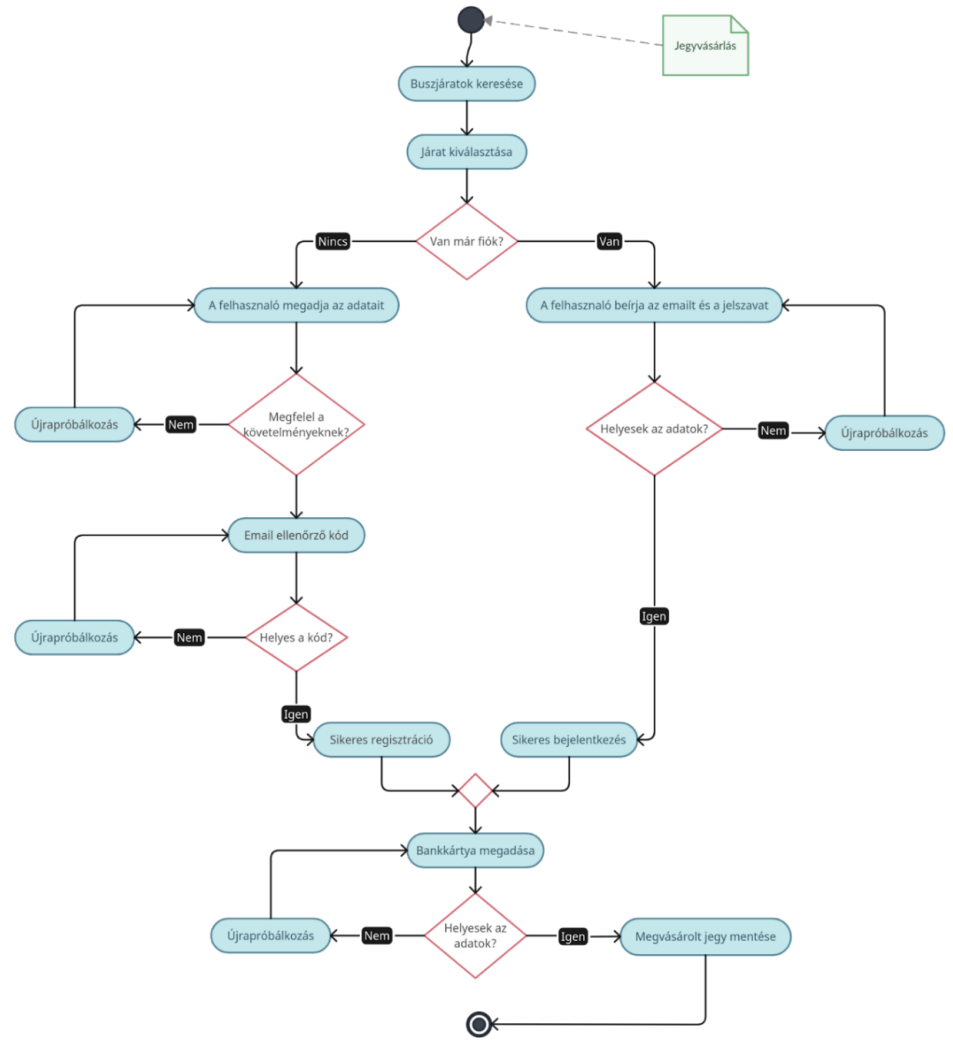
\includegraphics[width=\textwidth]{figures/activity.png}
    \caption{Aktivitás diagram az utazás tervezésének folyamatáról}
    \label{fig:activity-diagram}
\end{figure}

Ahogy a \ref{fig:activity-diagram} ábrán is látható, miután a felhasználó megtalálta a megfelelő
buszjáratot és rálépett a jegy(ek) megvásárlására, a rendszer átirányítja őt a
bejelentkezéshez, itt ha van már fiókja, bejelentkezhet a meglévő adataival,
amennyiben nincs, úgy átléphet a regisztrációs oldalra, ahol meg kell adnia a nevét,
email címét, és egy új jelszót. A rendszer minden adatot ellenőriz és ha valamelyik
hibás (pl. érvénytelen email cím vagy túl rövid jelszó) akkor egy hibaüzenetet ír ki. Ez
addig ismétlődik, amíg minden adat megfelelő lesz, aztán automatikusan küldünk egy
ellenőrző kódot a megadott e-mailre, amelyet a felhasználó be kell írjon a webes
felületen megjelenő szövegmezőbe.

\begin{figure}[H]
    \centering
    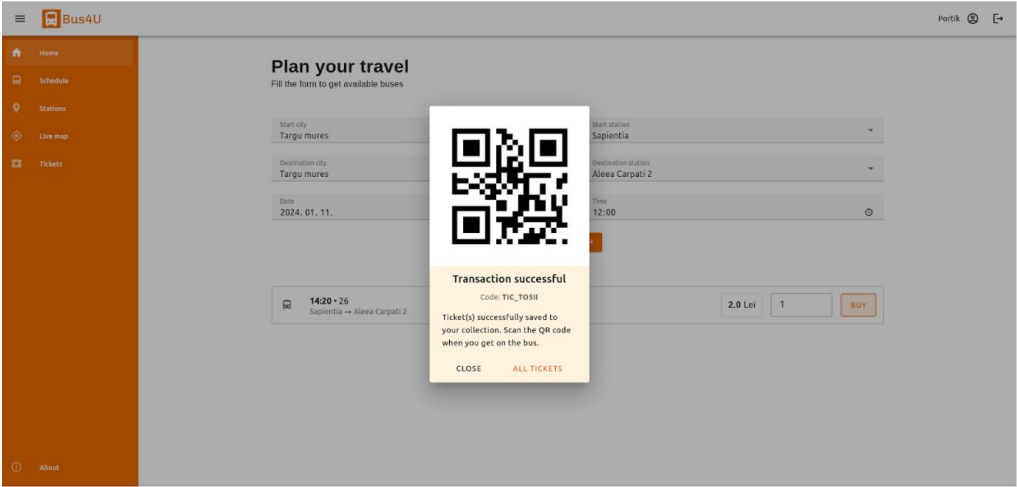
\includegraphics[width=\textwidth]{figures/boughtticket.png}
    \caption{Megvásárolt jegy}
    \label{fig:bought-ticket}
\end{figure}

Ha ez helytelen, ez is addig ismétlődik, amíg
minden rendben lesz, majd a rendszer átirányítja a felhasználót a bankkártyás
fizetéses oldalra, ami jelenleg nincs implementálva, ez a jövőbeli tervek között
szerepel. Ezután már csak az következik, hogy a rendszer elmenti a megvásárolt jegy
kódját, amelyet a felhasználó a Jegyek oldalon talál meg szöveges és QR-kódos
formátumban.

\begin{figure}[H]
    \centering
    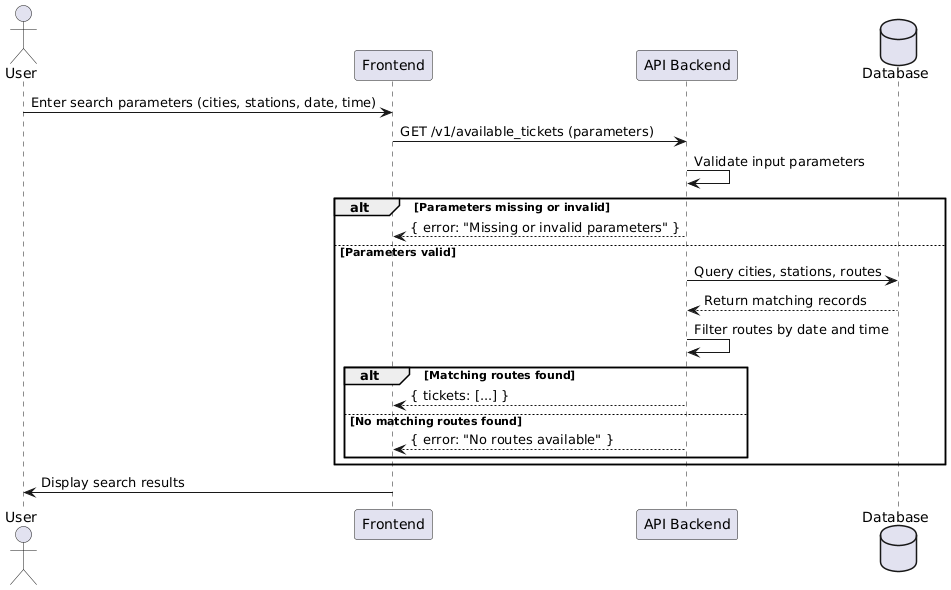
\includegraphics[width=\textwidth]{figures/listtickets.png}
    \caption{Szekvencia diagram az útvonaltervezés folyamatáról}
    \label{fig:seq-diagram-1}
\end{figure}

\subsection{Jegyek}
A megvásárolt jegyeket a rendszer elmenti a gyűjteménybe, ami a Jegyek oldalon
található, így a jegyek bármikor visszakereshetőek és felhasználhatóak lesznek,
kivéve ha lejár az egy hónapos érvényesség.

A jegyen megjelenített adatok között van
a járat neve, a kiinduló- és célállomás, az ár, valamint a vásárlás és az érvényesség
dátumai. A már elhasznált jegyek megvannak jelölve így azokat nem lehet többször
felhasználni.
A jegyeket QR-kód formájában is megjelenítjük ( \ref{fig:bought-ticket} ábra), amelyeket az utasok be tudnak szkennelni.

\begin{figure}[H]
    \centering
    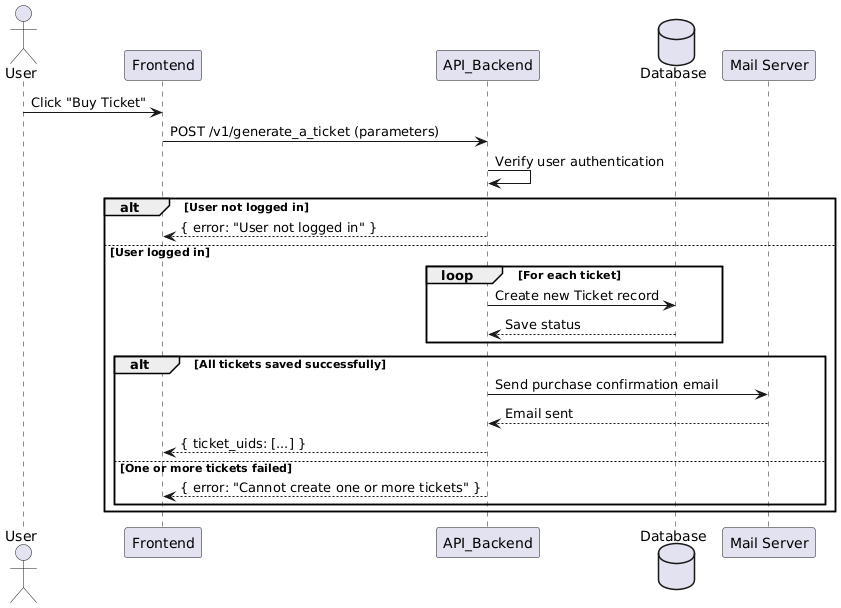
\includegraphics[width=\textwidth]{figures/buyticket.png}
    \caption{Szekvencia diagram a jegyvásárlás folyamatáról}
    \label{fig:seq-diagram-2}
\end{figure}

\subsection{Menetrend}
A következő oldal a menetrend, amely hasonlóan a buszmegállókban kihelyezett
táblázatokhoz, megjeleníti a kiválasztott buszjárat indulási időpontjait, az adott
megállóból. A mi megoldásunk viszont tartalmaz emellett egy térképet is, ahol meg
lehet nézni a járat útvonalát, az érintett megállókat és az útvonalon közlekedő buszok
élő pozícióját is.

\subsection{Megállók és térkép}
Ez a két oldal a fent említett térképes funkciókat mutatják meg külön-külön,
egyszerűbben. Egyik megjeleníti a térképen az összes megállót, és ezek között
szűrést is biztosít város vagy buszjárat szerint. A másik oldalon pedig egy-egy
útvonalon közlekedő buszok élő pozícióját lehet követni, miután kiválasztottuk a várost
és az útvonalat. Ez a funkció abban segít, hogy ne maradjunk le, ha egy busz siet,
illetve ne várakozzunk feleslegesen a megállóban, ha egy busz késik, így időt lehet
vele spórolni.

\section{Adminisztrációs felület}
Az admin felület csak bejelentkezéssel elérhető, ehhez egy admin rangú
felhasználói fiók szükséges, amely egy adott céghez van hozzárendelve. A cégek
adatai el vannak különítve, így minden admin csak a saját cégéhez tartozó adatokat
láthatja és módosíthatja.

\subsection{Kezdőlap}
Belépés után egy összegző oldal jelenik meg amelyen látható egy kis statisztika
a regisztrált felhasználók számával, a megvásárolt jegyek számával és a bevétellel,
mindez havi, évi és mindenkori bontásban. Itt jelennek meg az esetleges
figyelmeztetések és értesítések is, például a buszok lejárt útadója vagy a közelgő
műszaki vizsgálat.

\begin{figure}[H]
    \centering
    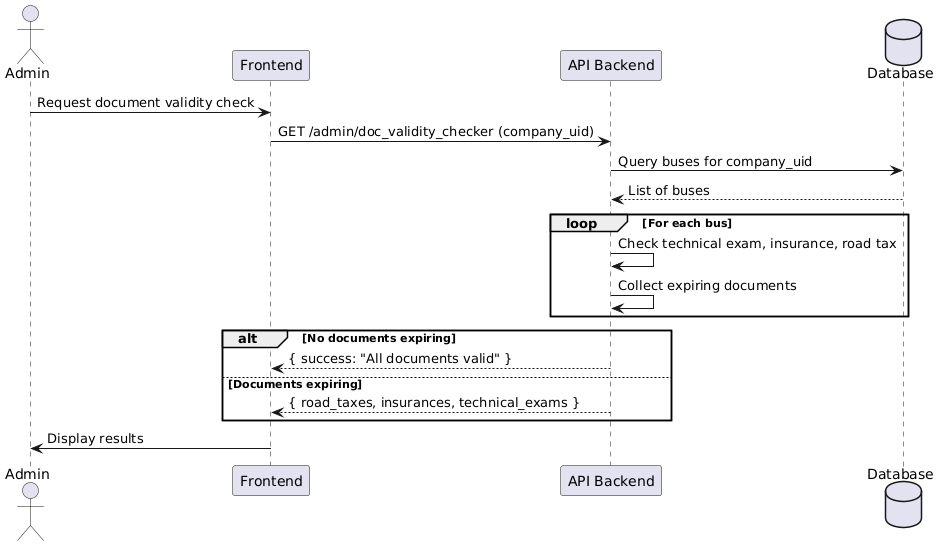
\includegraphics[width=\textwidth]{figures/checkdocuments.png}
    \caption{Szekvencia diagram a dokumentumok ellenőrzéséről}
    \label{fig:seq-diagram-3}
\end{figure}

\subsection{Megállók}
A Megállók oldalon létre lehet hozni új megállókat, megtekinteni meglévőket a
térképen vagy törölni ezeket. Új megálló hozzáadásához meg kell adni a megálló
nevét, a címet és a koordinátákat. A néven kívül, a többi adatot automatikusan kitölti a
rendszer, ha a térképen a megálló helyére kattint a felhasználó, de manuálisan is meg
lehet adni.

\subsection{Útvonalak}
Ezen az oldalon lehet felépíteni útvonalakat a létrehozott megállókból és itt lehet
megadni az alap jegyárat is, abban az esetben, ha a jegyek ára nem függ a megtett
távolságtól és időtől, hanem mindig és mindenhova ugyanannyi, ez esetben a fizetés
az útvonalhoz lesz hozzárendelve, nem a különböző megállókhoz.

\subsection{Menetrend}
A következő oldal a Menetrend, ahol a létrehozott útvonalak megállóihoz lehet
órarendeket hozzárendelni. Itt meg kell adni az órarendre érvényes napokat, a
következő megállóig szükséges jegyárat és az indulási időpontokat. Egy megállóhoz
hozzá lehet adni több ilyen órarendet is, ha különböző napokra különböző órarend
érvényes. Így el lehet választani a hétvégét a hétköznapoktól, ha mások az indulási
időpontok, vagy ha például hétvégén drágább a jegy.

\subsection{Buszok és alkalmazottak}
Az utolsó két oldalon a buszokat és az alkalmazottakat lehet kezelni. Hasonlóan
működnek, mindkettőn található egy lista a meglévő elemekkel, ahol bármelyiket lehet
módosítani vagy törölni, illetve újat is lehet létrehozni. A buszoknál meg kell adni a
márkát, a rendszámot, a férőhelyek számát, a gyártási évet, valamint az útadó, a
biztosítás és a műszaki engedély lejárati dátumát. Új alkalmazott hozzáadásánál meg
kell adni a nevet, e-mail címet, beosztást, telefonszámot, lakcímet (opcionális), és egy
új jelszavat.


\section{POS terminál alkalmazása}
\subsection{GPS oldal}
Miután a sofőr bejelentkezett, ezen
az oldalon lehetőség nyílik kiválasztani
az aktuális buszt, amelyiket jelenleg a
sofőr vezet, illetve azt az útvonalat,
amelyet éppenséggel végrehajt. Található egy kapcsoló, amellyel el lehet
indítani az autóbusz lokációjának
követését. Ez félpercenként küldi fel az
API-ra a busz lokációját, ezáltal lehet a
weboldalon és az alkalmazásban élőben
követni a busz helyzetét. Illetve ezen opció bekapcsolásakor megjelenik egy térkép is, amelyen élőben láthatjuk a busz pontos helyzetét.
Legalul egy Ticket scanner gomb fedezhető fel,
amely átirányít a jegyszkennelő oldalra

\begin{figure}[H]
    \centering
    \begin{minipage}{0.48\textwidth}
        \centering
        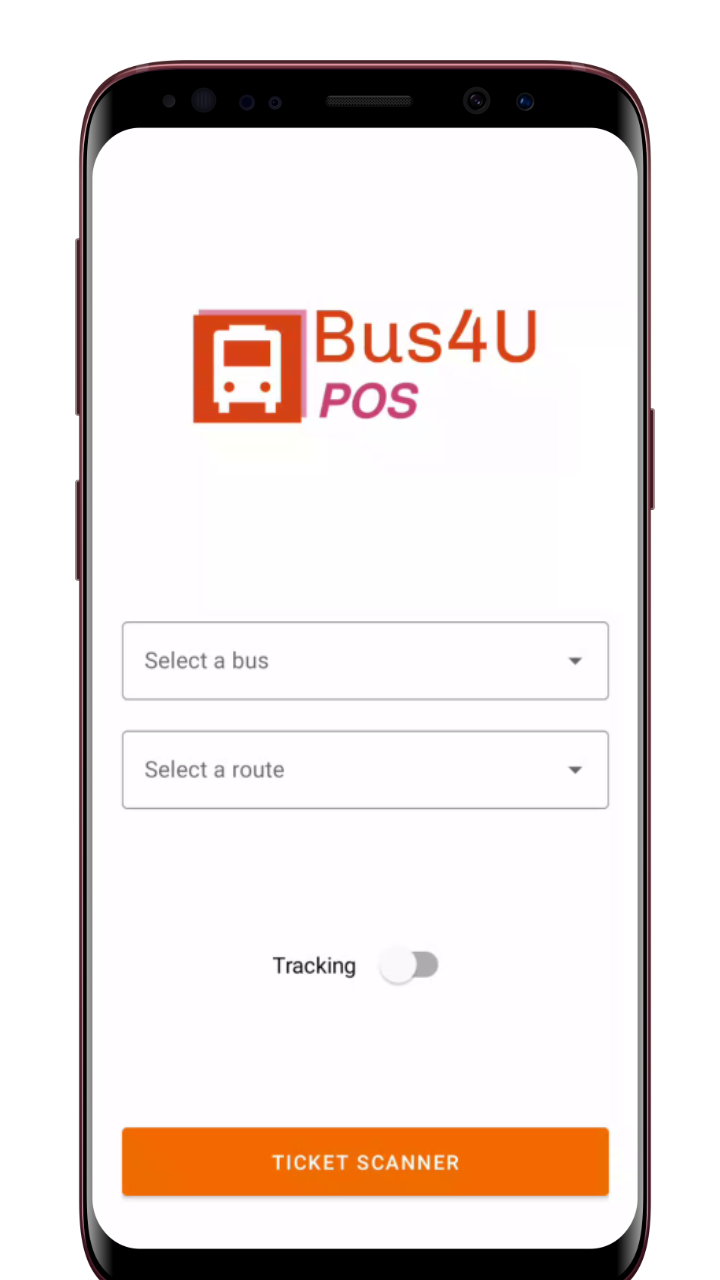
\includegraphics[width=\textwidth]{figures/pos_1.png}
        \caption{Busz kiválasztása és GPS követés}
        \label{fig:gps1}
    \end{minipage}\hfill
    \begin{minipage}{0.48\textwidth}
        \centering
        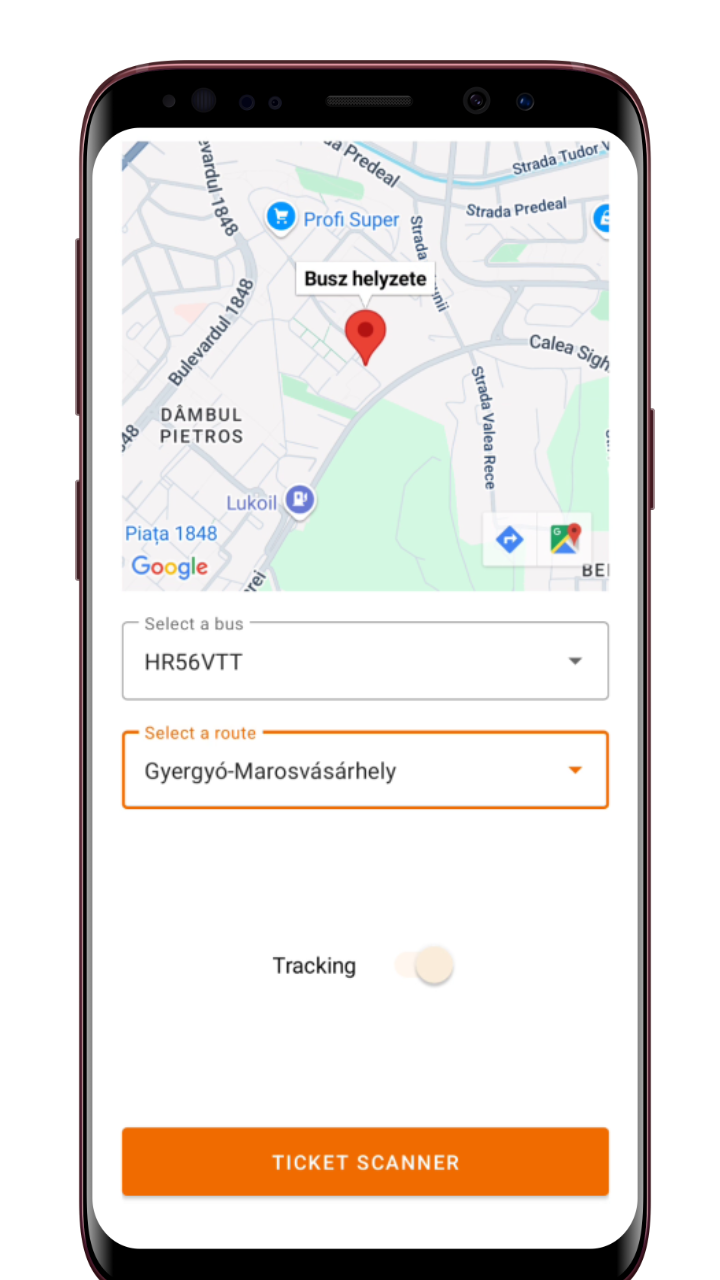
\includegraphics[width=\textwidth]{figures/pos_2.png}
        \caption{Elindított GPS követés}
        \label{fig:gps2}
    \end{minipage}
\end{figure}

\subsection{Jegyszkennelő oldal}
Ez az oldal a kamerát jeleníti meg.
Itt kell beszkennelni a jegyet. Szkennelés
után egy szöveges üzenet jelenik meg 5
másodpercig, három üzenetet hordozhat:
Ha sikeresen érvényesítve van a jegy,
akkor zöld háttérrel kiírja hogy sikeres
érvényesítés. Ha a jegy már érvényesítve
volt, vagy érvénytelen a QR kód, ezt egy
piros hibaüzenettel jelzi. Illetőleg ha az
API valamilyen oknál fogva leáll, akkor
ennek a hibájáról is üzenetet kapunk.

\begin{figure}[H]
    \centering
    \begin{minipage}{0.48\textwidth}
        \centering
        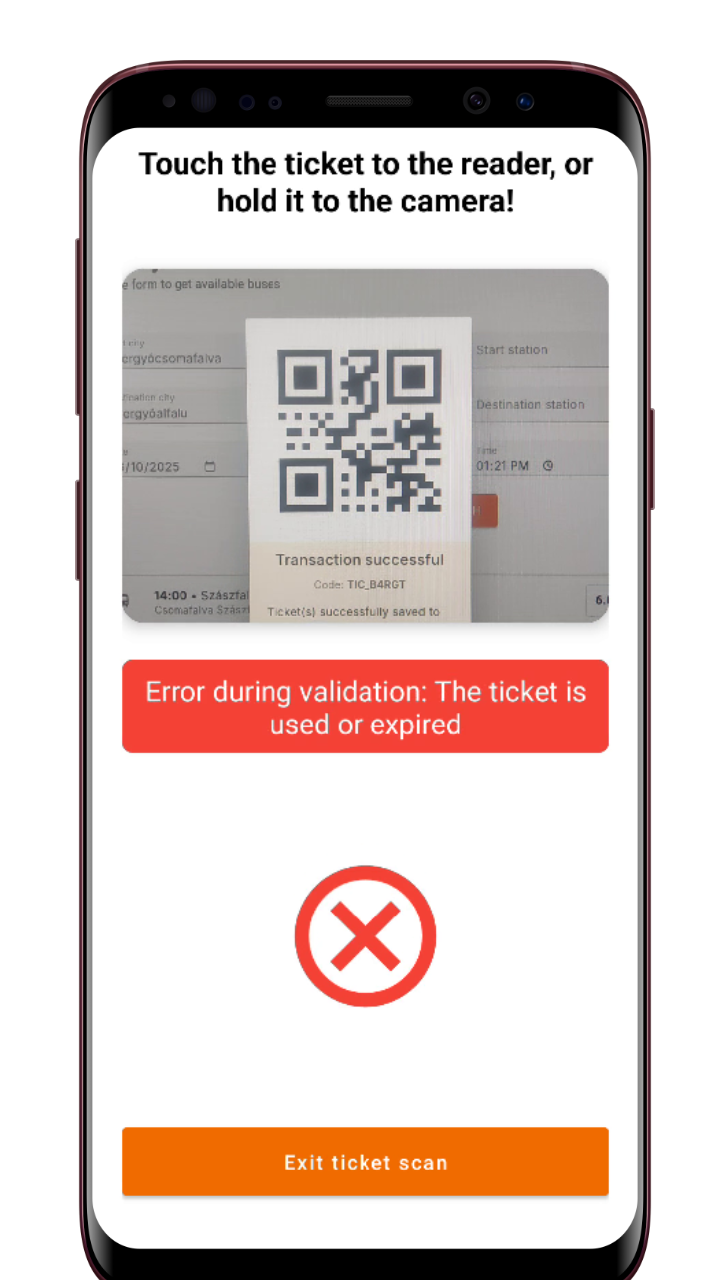
\includegraphics[width=\textwidth]{figures/pos_3.png}
        \caption{Sikeres jegy érvényesítés}
        \label{fig:pos_success}
    \end{minipage}\hfill
    \begin{minipage}{0.48\textwidth}
        \centering
        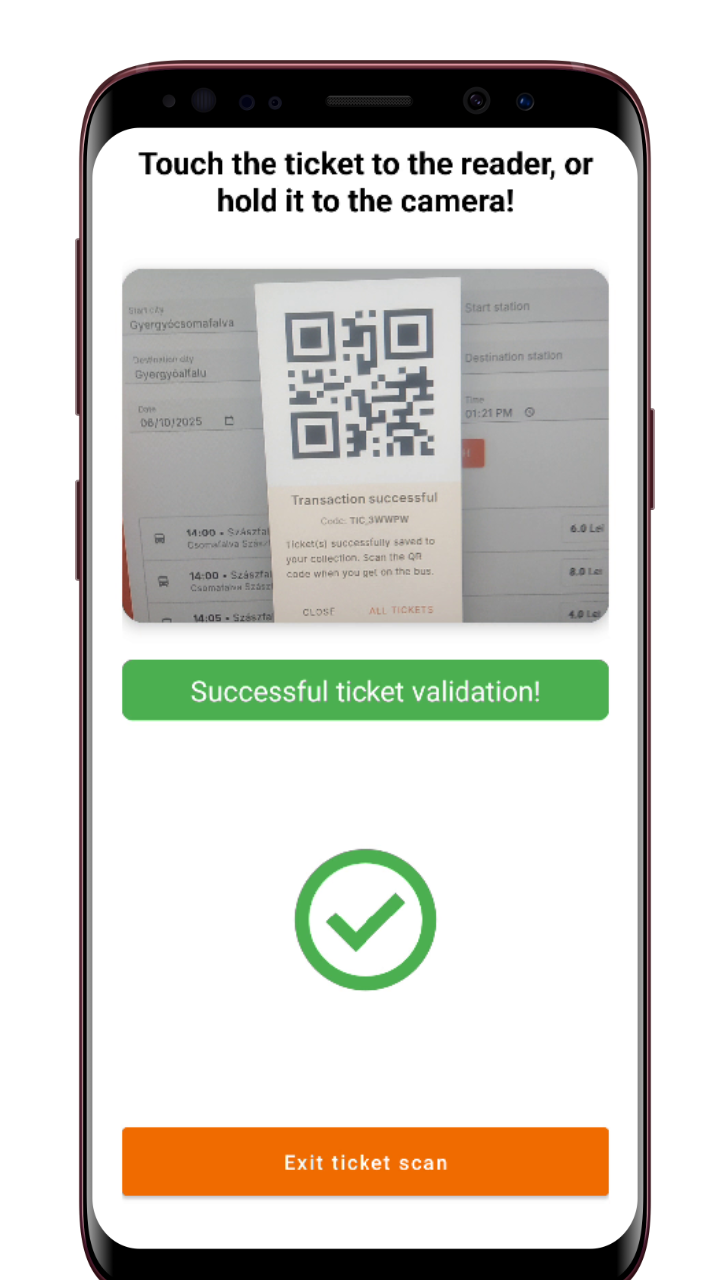
\includegraphics[width=\textwidth]{figures/pos_4.png}
        \caption{Sikertelen jegy érvényesítés}
        \label{fig:pos_error}
    \end{minipage}
\end{figure}

\chapter{A rendszer tesztelése}
\section{Tesztelési környezet}

A tesztelést egy helyi fejlesztési környezetben végeztem. A szerver a következő konfigurációval működött:
\begin{itemize}
    \item \textbf{Operációs rendszer:} Ubuntu 22.04 LTS
    \item \textbf{Szerver:} Ruby on Rails 7.0.4
    \item \textbf{Adatbázis:} PostgreSQL 14
    \item \textbf{Tesztelő eszköz:} Postman v10.0
\end{itemize}


\section{Funkcionális tesztelés}

A rendszer funkcionális teszteléséhez a Postman eszközt használtam. A Postman lehetőséget nyújt HTTP-kérések küldésére, valamint a különböző API végpontok működésének, válaszainak és adatstruktúráinak ellenőrzésére. Az alábbiakban bemutatom a tesztelés folyamatát és az eredményeket.

A tesztelést egy helyi fejlesztési környezetben végeztem, ahol a szerver a következő címen volt elérhető:

\begin{verbatim}
http://localhost:3000/api/v1/
\end{verbatim}

A Postman segítségével különböző HTTP metódusokat (GET, POST, PUT, DELETE) használtam a végpontok tesztelésére. Az egyes végpontokat a rendszer megfelelő válaszai alapján ellenőriztem.

\subsection{Végpontok tesztelése}

Az alábbi végpontok tesztelését szeretném kiemelni:

\begin{itemize}
    \item \textbf{GET {{api\_url}}/v1/get\_stations\_by\_city} – Lekéri az állomásokat a megadott város alapján.
    \item \textbf{GET /v1/get\_departure\_times\_for\_station\_in\_route} – Indulási időpontok lekérése egy adott járatra és állomásra.
    \item \textbf{GET /v1/get\_available\_tickets} – Elérhető jegyek lekérdezése az adott kiindulási és célállomásra.
    \item \textbf{GET /v1/get\_bus\_locations\_by\_route} – A buszok aktuális helyzetének lekérése egy adott járatra.
    \item \textbf{GET /v1/tickets\_of\_user} – Az aktuális felhasználó jegyeinek lekérése.
    \item \textbf{GET /v1/admin/document\_validity\_checker} – Dokumentum érvényességének ellenőrzése adminisztrátorok számára.
    \item \textbf{GET /v1/admin/statistics} – Statisztikai adatok lekérdezése egy adott cég számára.
\end{itemize}


\subsection{Tesztelési példa}

Például a GET metódus használatával kértem le az állomásokat egy megadott város alapján:

\begin{verbatim}
GET api.bus4u.online/v1/get_stations_by_city?city_uid=CTY_N11XH
\end{verbatim}

A szerver válasza a következő JSON formátumban érkezett:

\begin{verbatim}
{
    "stations": [
        {
            "station_uid": "STT_EGAVX",
            "name": "Sapientia",
            "address": "Str. Calea Sighisoarei nr. 2",
            "longitude": "24.59883",
            "latitude": "46.52339"
        },
        {
            "station_uid": "STT_6CO3Q",
            "name": "Dedeman",
            "address": "Bul. 1 Decembrie nr. 189",
            "longitude": "24.59941",
            "latitude": "46.52678"
        }
    ]
}
\end{verbatim}

Ezzel a lekérdezéssel sikeresen megkaptam az adatokat, amelyeket a rendszer helyesen dolgozott fel.

\subsection{Tesztelési eredmények}

A tesztelés során az összes végpontot felvezettem Postman-re, és mindegyik megfelelően működött. Az egyes végpontok válaszai megfeleltek az elvárt adatstruktúrának, és a rendszer helyesen kezelte a kéréseket.


\section{Teljesítménytesztelés}
A teljesítménytesztelés célja a rendszer stabilitásának és skálázhatóságának értékelése volt nagy terhelés alatt. A vizsgálat során a JMeter eszközt használtam, amely képes különböző mennyiségű egyidejű felhasználói kérések szimulálására.

A JMeter mintavételi eredményei alapján az alábbi teljesítménymetrikák és azok jelentőségeit vizsgáljuk az API teljesítményével kapcsolatban:

\subsection{Teljesítmény-metrikák}
KIEGÉSZÍTENI AZ ÚJRATESZTELT ADATOKKAL


\section{Biztonsági tesztelés}
A biztonsági tesztelés során különös figyelmet fordítottam a következő sebezhetőségek elkerülésére:
\begin{itemize}
    \item \textbf{SQL injection} – Input validálás és előkészített SQL lekérdezések használata.
    \item \textbf{Cross-site scripting (XSS)} – HTML entitások kódolása a felhasználói bemeneteknél.
    \item \textbf{Cross-site request forgery (CSRF)} – CSRF tokenek használata minden kényes műveletnél.
\end{itemize}

\section{Összegzés}
A tesztelési eredmények alapján a rendszer minden funkciója megfelelően működik, a teljesítménye kielégítő, és a biztonsági mechanizmusok jól védik az API-t a lehetséges támadások ellen. A további tesztelések célja az API skálázhatóságának javítása, valamint az integrációs lehetőségek vizsgálata más külső rendszerekkel.



\chapter{Összefoglalás}
Ez a fejezet összefoglalja a Bus4U rendszer API-jának tervezését, megvalósítását és tesztelését, valamint bemutatja a legfontosabb megállapításokat és javaslatokat a jövőbeli fejlesztésekhez.

A dolgozat célja egy hatékony busz menedzselő rendszer API létrehozása volt, amely lehetővé teszi a felhasználók számára a buszjáratok, jegyek és bérletek kezelését, valamint a rendszeres frissítéseket és karbantartásokat. A projekt során a következő lépéseket tettük:

1. Követelmények és tervezés: A rendszer funkcionális és nem funkcionális követelményeinek részletes elemzése és a legfontosabb funkciók prioritásának meghatározása. A követelmények alapján a rendszer architektúráját és az API felépítését terveztük meg.

2. API megvalósítása: Az API endpointok megvalósítása során külön figyelmet fordítottunk a RESTful architektúra elveinek betartására, biztosítva ezzel a könnyű használhatóságot és a skálázhatóságot. A végpontok különböző erőforrásokat (buszok, járatok, jegyek, bérletek) kezelnek, lehetővé téve a felhasználók számára, hogy egyszerűen hozzáférjenek az információkhoz és végrehajtsanak műveleteket.

3. Tesztelés: A rendszer tesztelését Postman segítségével végeztük, ahol különböző kéréseket küldtünk az API végpontokhoz, hogy ellenőrizzük azok működését, a válaszok helyességét és a teljesítményt. A tesztelési folyamat során sikerült azonosítani és javítani a hibákat, így a rendszer stabil és megbízható lett.

4. Deployment: A rendszer telepítése az Azure felhőszolgáltatásra történt, ahol az API az api.bus4u.online domainen érhető el. A PostgreSQL adatbázis és a virtuális gép (VM) külön szolgáltatásként működik, biztosítva a skálázhatóságot és a megbízhatóságot.

5. Jövőbeli fejlesztések: A jövőbeli fejlesztések között szerepel a rendszer funkcionalitásának bővítése, például új szolgáltatások bevezetése, a felhasználói élmény javítása érdekében. További cél a rendszer biztonságának növelése, például a hitelesítési és jogosultsági mechanizmusok fejlesztésével.

Összességében a Bus4U API megvalósítása sikeres volt, és a dolgozat során végrehajtott lépések hozzájárultak a hatékony és megbízható busz menedzselő rendszer kialakításához. A projekt során szerzett tapasztalatok és tanulságok értékes alapot jelentenek a jövőbeli fejlesztésekhez és a hasonló rendszerek tervezéséhez.


\addcontentsline{toc}{chapter}{Irodalomjegyzék}
\bibliographystyle{ieeetr}
\bibliography{references}

\appendix
\chapter{Függelék}
\input{chapters/appendix}

\end{document}